This section aims to join every results obtained in the last chapter in order to give a unique score for each heuristic section. This is done by computing the arithmetic average of the scores of \textit{Navigation}, \textit{Contents} and \textit{Layout} sections.\par
\bigskip
\section{Scores}
\subsection{MiLE}
\textbf{Navigation}\par
The navigation score is given by the mean of the 5 aspects analyzed in the section \ref{Navigation}. \par 
The final result is: 
(4.5 + 4.5 + 4 + 3.5 + 3.5)/5 = \textbf{4}\par
Therefore, content aspect in the Moviri website is handled well, even if could be improved again.

\begin{figure}[H]
  \centering
  \makebox[\linewidth]{
    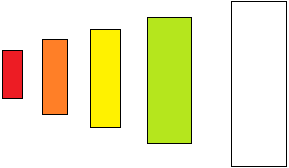
\includegraphics[scale=0.35]{images/4.png}}
\end{figure}

\par\medskip

\textbf{Contents}\par
The score of this section is given simply by the score evaluated by the \textit{Information Overload} heuristic which is \textbf{4.5}. \par
So basing only this heuristic, content of the website is almost fully satisfied. Improvements could be done, but fixes will be minimal.

\begin{figure}[H]
  \centering
  \makebox[\linewidth]{
    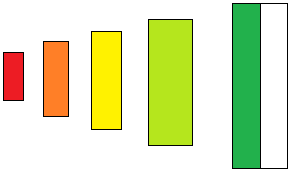
\includegraphics[scale=0.35]{images/4.5.png}}
\end{figure}


\par\medskip

\textbf{Layout}\par
The layout score is given by the mean of 5 aspects analyzed in the section \ref{Layout}. \par
The final result is: 
(4 + 4 + 4 + 4 + 3)/5 = 3.8 \\
\textit{which can be approximated to} \textbf{4}\par
Basing on the result, layout of the website it's pretty well designed, but with some critical issues that should be fixed in order to have the best experience.

\begin{figure}[H]
  \centering
  \makebox[\linewidth]{
    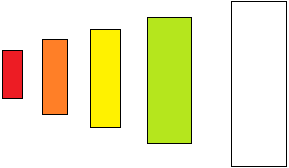
\includegraphics[scale=0.35]{images/4.png}}
\end{figure}


\subsection{Nielsen}
Instead, the evaluation with this set of heuristics is made by making the average of all the six heuristcs analyzed:
(2 + 4 + 3.5 + 4 + 5 + 4.5)/6 = 3.8 \\
\textit{which can be approximated to} \textbf{4}.\par

\section{Comments}
